\section{受迫响应}
\label{sec:heat-forced}

前面的解都由初值产生。如果棒上有持续的热源，或者端点的温度随时间改变，解又是什么？方程是线性的，答案的思路只有一条：把外部输入切成小片，每一片都当成一次自由演化的起点，再叠加起来。

\paragraph{从常微分方程到扩散}
线性常微分方程$\dot{\bm{x}}=\bm{A}\bm{x}+\bm{g}(t)$的解是
\[
 \bm{x}(t)=\mathrm{e}^{t\bm{A}}\bm{x}_0+\int_0^t\mathrm{e}^{(t-s)\bm{A}}\bm{g}(s)\,\mathrm{d}s .
\]
积分号下的读法是：时刻$s$注入的增量$\bm{g}(s)\,\mathrm{d}s$随后按齐次方程走了$t-s$的时间。

扩散的情形完全一样。时间片$[s,s+\Delta s]$内注入的热量分布大约是$f(\cdot,s)\Delta s$，它接下来自由扩散$t-s$的时间。把所有时间片的贡献加起来，令$\Delta s\to0$，得到\term{Duhamel公式}（Duhamel formula）。

\paragraph{全空间的表示}
对全空间，自由扩散由热核给出，于是
\begin{equation}
 u(\bm{x},t)=\int_{\mathbb{R}^{d}}G(\bm{x}-\bm{y},t)\,u_0(\bm{y})\,\mathrm{d}\bm{y}+\int_0^t\!\!\int_{\mathbb{R}^{d}}G(\bm{x}-\bm{y},t-s)\,f(\bm{y},s)\,\mathrm{d}\bm{y}\,\mathrm{d}s .
 \label{eq:heat-duhamel-space}
\end{equation}
图~\ref{fig:heat-duhamel-pulses}取$\lvert x\rvert<1/4$上的单位热源，持续到$t=0.5$，切成五片。较晚注入的片（深色）还很集中，较早注入的已经散开，它们的和（绿点）贴近精确的积分（蓝）。

\begin{BookInlineFigure}
  \centering
  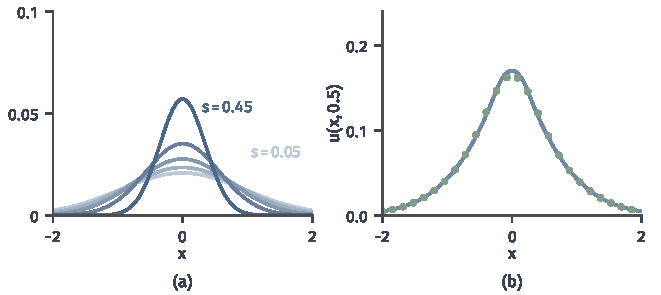
\includegraphics[width=112mm]{figures/06-differential-equations/02-partial-differential-equations/matplotlib/heat-duhamel-pulses/figure.pdf}
  \caption{热源$f=\mathbb{I}_{[-1/4,1/4]}(x)$，$0<s<0.5$，初值为零，观察时刻$t=0.5$。(a)五个时间片（$s=0.05,0.15,\ldots,0.45$，$\Delta s=0.1$）各自的响应，颜色越深注入越晚。(b)五片之和（绿点）与时间积分的精确结果（蓝）。}
  \label{fig:heat-duhamel-pulses}
\end{BookInlineFigure}

把这个想法变成定理，难点在$s\to t$时核变成奇异的。只要把时间积分靠近奇异点的一段切开，用热核收回初值的性质来处理。

\begin{theorem}[全空间的Duhamel公式]
\label{thm:heat-duhamel-space}
设$f$及其导数$\partial_tf$、$\partial_{x_i}f$、$\partial_{x_i}\partial_{x_j}f$在$\mathbb{R}^{d}\times[0,T]$上有界连续，并取$u_0=0$。则式~\eqref{eq:heat-duhamel-space}的第二项给出的$u$在$\mathbb{R}^{d}\times(0,T]$上有连续的$\partial_tu$与二阶空间偏导，并满足
\begin{equation}
 \partial_tu=\Delta u+f,\qquad \lim_{t\to0^+}\sup_{\bm{x}}\lvert u(\bm{x},t)\rvert=0 .
 \label{eq:heat-duhamel-solves}
\end{equation}
\end{theorem}

\begin{proof}
由$\int G=1$，$\lvert u(\bm{x},t)\rvert\leq t\sup\lvert f\rvert$，这给出初值条件。

为了求导，先把$\bm{y}$和$s$都换成相对量，令$\bm{y}\mapsto\bm{x}-\bm{y}$、$s\mapsto t-s$：
\[
 u(\bm{x},t)=\int_0^t\!\!\int G(\bm{y},s)\,f(\bm{x}-\bm{y},t-s)\,\mathrm{d}\bm{y}\,\mathrm{d}s .
\]
现在$\bm{x}$和$t$只出现在光滑的$f$中，可以在积分号下求导：
\[
 \Delta u=\int_0^t\!\!\int G(\bm{y},s)\,\Delta f(\bm{x}-\bm{y},t-s)\,\mathrm{d}\bm{y}\,\mathrm{d}s,
\]
\[
 \partial_tu=\int_0^t\!\!\int G(\bm{y},s)\,\partial_tf(\bm{x}-\bm{y},t-s)\,\mathrm{d}\bm{y}\,\mathrm{d}s+\int G(\bm{y},t)f(\bm{x}-\bm{y},0)\,\mathrm{d}\bm{y} .
\]
记$F(\bm{y},s)=f(\bm{x}-\bm{y},t-s)$，则$\partial_tf=-\partial_sF$，$\Delta f=\Delta_{\bm{y}}F$。相减，并把时间积分在小的$\varepsilon>0$处切开：
\[
 (\partial_t-\Delta)u=\int_\varepsilon^t\!\!\int G\,(-\partial_s-\Delta_{\bm{y}})F\,\mathrm{d}\bm{y}\,\mathrm{d}s+R_\varepsilon+\int G(\bm{y},t)F(\bm{y},t)\,\mathrm{d}\bm{y},
\]
其中$R_\varepsilon$是$[0,\varepsilon]$上的积分，由导数有界，$\lvert R_\varepsilon\rvert\leq C\varepsilon$。

第一项在$[\varepsilon,t]$上对$s$和$\bm{y}$分部积分，这里$G$光滑且快速衰减，边界只出现在$s=\varepsilon$和$s=t$：
\[
 \int_\varepsilon^t\!\!\int(\partial_sG-\Delta G)F\,\mathrm{d}\bm{y}\,\mathrm{d}s+\int G(\bm{y},\varepsilon)F(\bm{y},\varepsilon)\,\mathrm{d}\bm{y}-\int G(\bm{y},t)F(\bm{y},t)\,\mathrm{d}\bm{y} .
\]
第一个积分为零，最后一项恰好与前面的$\int G(\bm{y},t)F(\bm{y},t)\,\mathrm{d}\bm{y}$抵消。于是
\[
 (\partial_t-\Delta)u=\int G(\bm{y},\varepsilon)f(\bm{x}-\bm{y},t-\varepsilon)\,\mathrm{d}\bm{y}+R_\varepsilon .
\]
令$\varepsilon\to0^+$。$f$有界且导数有界，所以一致连续，用定理~\ref{thm:heat-uniform-recovery}同样的分段估计，右端趋于$f(\bm{x},t)$。导数的连续性由积分号下的表达式得到。
\end{proof}

这里要求$f$光滑，是因为导数都放在了$f$上。降低$f$的正则性时，经典解可能不存在，式~\eqref{eq:heat-duhamel-space}仍然可以作为一个积分定义的解，这一点在解半群一节再说。

\begin{example}[恒定点源]
\label{ex:heat-line-point-source}
实轴原点处有单位强度的恒定点源，初值为零。它不满足定理的光滑要求，但式~\eqref{eq:heat-duhamel-space}中的积分仍有意义，给出$u(x,t)=\int_0^tG(x,s)\,\mathrm{d}s$。在原点，
\[
 u(0,t)=\int_0^t\frac{\mathrm{d}s}{\sqrt{4\pi s}}=\sqrt{\frac{t}{\pi}} .
\]
$t=1$时为$0.5642$，$t=4$时为$1.1284$，无限增长。实轴上一维的点源没有稳态，因为热量散开的速度跟不上注入的速度。
\end{example}

图~\ref{fig:heat-line-point-source}对比了这一点。区间上情形不同。在$(0,1)$的中点放同样的单位点源，两端保持为零，温度有界，稳态是折线$\tfrac12\min\{x,1-x\}$，中点的值是$1/4$：吸热的端点把注入的热量带走了。

\begin{BookInlineFigure}
  \centering
  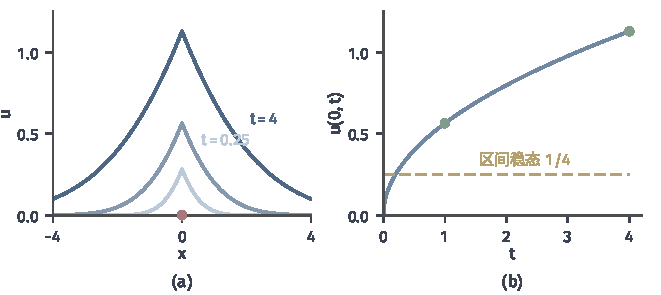
\includegraphics[width=112mm]{figures/06-differential-equations/02-partial-differential-equations/matplotlib/heat-line-point-source/figure.pdf}
  \caption{实轴上原点处的恒定单位点源（红点）。(a)$t=0.25,1,4$时的温度（蓝色由浅到深），原点处有一个折角。(b)原点温度$\sqrt{t/\pi}$（蓝）无限增长，绿点是$t=1,4$的值；黄色虚线是$(0,1)$上中点受单位点源、两端为零时的稳态值$1/4$。}
  \label{fig:heat-line-point-source}
\end{BookInlineFigure}

\paragraph{边界模式的表示}
在区间上自由演化由模式给出，同样的切片思想逐个模式进行。设$u$按$e_k$展开，系数记为$a_k(t)$，$f_k(t)=\langle f(\cdot,t),e_k\rangle$。用$e_k$检验$\partial_tu=\partial_x^2u+f$，分部积分两次，端点项因零边值而消失，每个模式得到一个独立的标量方程：
\[
 a_k'(t)=-\lambda_ka_k(t)+f_k(t) .
\]
这是一个标准的一阶线性方程，解出
\begin{equation}
 a_k(t)=\mathrm{e}^{-\lambda_kt}a_k(0)+\int_0^t\mathrm{e}^{-\lambda_k(t-s)}f_k(s)\,\mathrm{d}s .
 \label{eq:heat-duhamel-modes}
\end{equation}

把系数合起来，并定义区间上的核
\begin{equation}
 G_D(x,y,t)=\sum_{k\geq1}e_k(x)e_k(y)\mathrm{e}^{-\lambda_kt},
 \label{eq:heat-dirichlet-kernel}
\end{equation}
式~\eqref{eq:heat-duhamel-modes}就写成了与式~\eqref{eq:heat-duhamel-space}同样的形状，只是$G(x-y,t-s)$换成了$G_D(x,y,t-s)$。这个核依赖$x$和$y$两个变量，不只是它们的差，因为端点破坏了平移不变性。

当$f:[0,T]\to L^2(0,1)$连续时，由$\lvert\int_0^t\mathrm{e}^{-\lambda_k(t-s)}f_k\,\mathrm{d}s\rvert$的Cauchy--Schwarz估计，级数在$L^2$中收敛，定义了一个$L^2$值的解。若$f$、$\partial_xf$、$\partial_x^2f$在$[0,1]\times[0,T]$上连续且$f$在端点为零，分部积分两次给出$\sup_s\lvert f_k(s)\rvert\leq C/k^2$。又由时间积分的直接估计，
\[
 \lambda_k\Bigl\lvert\int_0^t\mathrm{e}^{-\lambda_k(t-s)}f_k(s)\,\mathrm{d}s\Bigr\rvert\leq\sup_s\lvert f_k(s)\rvert .
\]
于是$\sum_k\lambda_k\lvert a_k\rvert$的受迫部分可和，级数可以逐项求导，得到经典解。

\begin{example}[恒定热源趋于稳态]
\label{ex:heat-source-steady}
在$(0,1)$上取$f=1$，$u_0=0$，两端为零。系数为
\[
 f_k=\sqrt2\int_0^1\sin(k\pi x)\,\mathrm{d}x=\frac{\sqrt2\,(1-(-1)^k)}{k\pi},
\]
奇数$k$上等于$2\sqrt2/(k\pi)$，偶数$k$上为零。由式~\eqref{eq:heat-duhamel-modes}，对恒定的$f_k$积分，
\[
 a_k(t)=\frac{f_k}{\lambda_k}\bigl(1-\mathrm{e}^{-\lambda_kt}\bigr) .
\]
$t\to\infty$时$a_k\to f_k/\lambda_k$，这正是$-u''=1$、零边值的稳态解$x(1-x)/2$的系数，$-\partial_x^2$在模式坐标中就是乘以$\lambda_k$。在中点，稳态值是$1/8$。
\end{example}

这个$f$在端点不为零，上面逐项求导的充分条件不适用，但解可以直接写成稳态减去自由衰减：
\[
 u=\frac{x(1-x)}{2}-\sum_k\frac{f_k}{\lambda_k}\mathrm{e}^{-\lambda_kt}e_k .
\]
第一项是多项式，第二项属于定理~\ref{thm:heat-series}的情形，所以$t>0$时仍是经典解。

中点的值由这个级数算出，$t=0.05,0.1,0.2,0.5$时依次是
\[
 0.0463,\quad 0.0769,\quad 0.1071,\quad 0.1241 .
\]
图~\ref{fig:heat-source-steady}(b)说明每个模式按自己的速度靠近稳态，最慢的是$k=1$，高频模式几乎立刻到位。

\begin{BookInlineFigure}
  \centering
  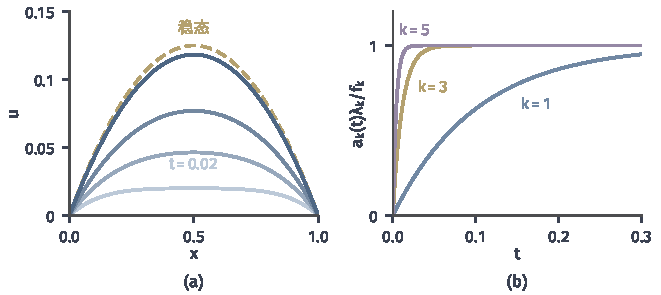
\includegraphics[width=112mm]{figures/06-differential-equations/02-partial-differential-equations/matplotlib/heat-source-steady/figure.pdf}
  \caption{恒定热源$f=1$，零边值，零初值。(a)$t=0.02,0.05,0.1,0.3$的解（蓝色由浅到深）趋于稳态$x(1-x)/2$（黄色虚线）。(b)各模式到稳态的比例$a_k(t)\lambda_k/f_k=1-\mathrm{e}^{-\lambda_kt}$，$k=1,3,5$。}
  \label{fig:heat-source-steady}
\end{BookInlineFigure}

\paragraph{非齐次边界的提升}
模式展开依赖零边值：分部积分时端点项才会消失。端点温度$u(0,t)=g_0(t)$、$u(1,t)=g_1(t)$非零时，先减去一个满足边界条件的函数，这称为\term{边界提升}（boundary lifting）。

设$g_0,g_1\in C^1[0,T]$，取线性插值
\[
 w(x,t)=(1-x)g_0(t)+xg_1(t) .
\]
令$v=u-w$。于是$v$在两端为零，而$\partial_x^2w=0$，代入原方程得到
\begin{equation}
 \partial_tv=\partial_x^2v+f-\partial_tw,\qquad v(x,0)=u_0(x)-w(x,0) .
 \label{eq:heat-lift-problem}
\end{equation}
边值变化的代价是多了一项源$-\partial_tw$，这就是要求$g_0,g_1$可微的原因。$v$现在可以用式~\eqref{eq:heat-duhamel-modes}求解。

Neumann情形要求端点斜率分别为$g_0$、$g_1$，提升不能用线性函数，因为一条直线只有一个斜率。取二次函数
\[
 w=g_0x+\frac{g_1-g_0}{2}x^2 ,
\]
这时$\partial_x^2w=g_1-g_0$不为零，$v=u-w$的源项是$f+\partial_x^2w-\partial_tw$。多维区域上可以用第~\ref{chap:elliptic-equations}章的调和函数作提升：取$\Delta w=0$、边界上$w=g$，再按上面的方式处理。

\begin{example}[一端突然加热]
\label{ex:heat-boundary-lift}
取$u_0=0$，$u(0,t)=0$，$u(1,t)=1$。提升函数是$w=x$，不随时间变化，于是$v$满足无源的热方程，初值$-x$。$x$在$e_k$上的坐标是$\sqrt2(-1)^{k+1}/(k\pi)$，所以
\[
 u(x,t)=x+\sum_{k\geq1}\frac{2(-1)^k}{k\pi}\,\mathrm{e}^{-k^2\pi^2t}\sin(k\pi x) .
\]
在中点，$t=0.05,0.1,0.2,0.5$的温度分别是
\[
 0.1138,\quad 0.2628,\quad 0.4116,\quad 0.4954 ,
\]
趋于稳态$w(1/2)=1/2$。
\end{example}

这个例子的初值和边值在$(1,0)$处矛盾，$v$的初值$-x$在$x=1$不为零，所以属于定理~\ref{thm:heat-series}的$L^2$情形，$t>0$时光滑。图~\ref{fig:heat-boundary-lift}中，(a)是$v$的衰减，(b)是加回$w$之后的$u$。

\begin{BookInlineFigure}
  \centering
  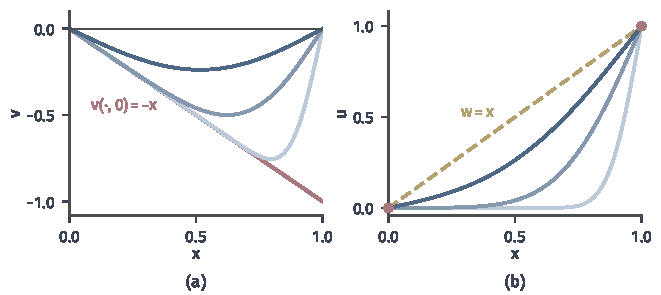
\includegraphics[width=112mm]{figures/06-differential-equations/02-partial-differential-equations/matplotlib/heat-boundary-lift/figure.pdf}
  \caption{边界提升，$u(0,t)=0$，$u(1,t)=1$，$u_0=0$，$t=0.005,0.03,0.1$（蓝色由浅到深）。(a)$v=u-w$，初值$-x$（红），两端为零。(b)$u=w+v$，黄色虚线是提升函数$w=x$，红点是边值。}
  \label{fig:heat-boundary-lift}
\end{BookInlineFigure}

\paragraph{全空间公式不能照搬}
既然有了卷积公式，能否直接把区间上的初值代进去？把三角形延拓成零，用实轴的核做卷积，图~\ref{fig:heat-wholeline-vs-interval}(a)的黄线就是结果。在$t=0.05$时它在端点的值约$0.111$，并不等于边值$0$，棒外的“真空”也被当成了可以吸收热量的材料。

对有特殊几何的区间，可以用\term{像源法}（method of images）修正。把初值奇延拓，再按周期$2$延拓，图~\ref{fig:heat-wholeline-vs-interval}(b)的红线就是这个延拓。这个函数在$x=0,1$两侧反对称，实轴上的卷积保持对称性，所以解在这些点始终为零。

\begin{BookInlineFigure}
  \centering
  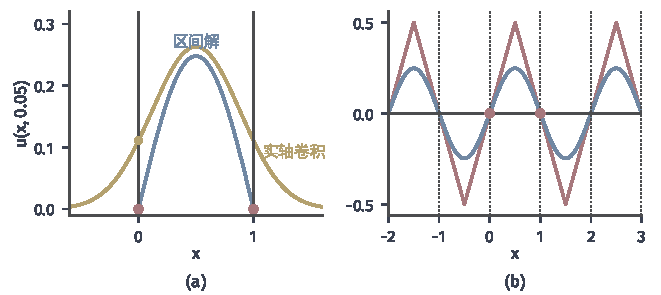
\includegraphics[width=112mm]{figures/06-differential-equations/02-partial-differential-equations/matplotlib/heat-wholeline-vs-interval/figure.pdf}
  \caption{实轴卷积与区间问题，三角形初值，$t=0.05$。(a)区间解（蓝）在端点（红点）为零；把三角形延拓为零后的实轴卷积（黄）在端点的值约$0.111$。深灰竖线是棒的端点。(b)奇延拓并按周期$2$延拓的初值（红）与实轴卷积（蓝），解在每个整数点为零。}
  \label{fig:heat-wholeline-vs-interval}
\end{BookInlineFigure}

用公式写出来，把周期延拓代入卷积，就得到另一种形式的区间核：
\begin{equation}
 G_D(x,y,t)=\sum_{n\in\mathbb{Z}}\bigl(G(x-y+2n,t)-G(x+y+2n,t)\bigr) .
 \label{eq:heat-image-kernel}
\end{equation}
它和式~\eqref{eq:heat-dirichlet-kernel}是同一个函数的两种写法，因为两者给出同一个问题的解，而解是唯一的，唯一性在第~\ref{sec:heat-properties}节证明。像源的写法在$t$小时收敛极快，只需$n=0$的项；模式的写法在$t$大时收敛极快，只需前几项。对图中的例子数值计算$u(1/2,0.05)$，两种写法都得到$0.24796$。一般区域没有这种反射结构，边界的作用需要由模式或其他方法处理。
